\chapter{Modelle von Motorr\"adern}\label{ch:modell}
Die Modellierung von Motorr\"adern ist Gegenstand aktueller Forschung. Insbesondere die Arbeiten von R. S. Sharp \cite{Sharp1971}, \cite{SHARP1985}, \cite{Sharp2001} sowie die Arbeiten von V. Cossalter und R. Lot \cite{Cossalter2002}, \cite{Cossalter2010} werden vielfach zitiert. Eine \"Ubersicht \"uber die historische Entwicklung von Motorradmodellen und zahlreiche Quellen sind in \cite{Limebeer2006} zu finden. Au\ss{}erdem liefert \cite{Schwab2013} eine umfangreiche Quellen\"ubersicht zur Modellierung und dem Fahrverhalten von Einspurfahrzeugen. Weitere aktuelle Modelle sind unter anderem in \cite{Kanoh2007}, \cite{Nehaoua2013}, dem umfangreichen Buch von M. Tanelli \cite{MaraTanelli2014a} und \cite{Leonelli2015} dargestellt. Zus\"atzlich sei noch das Buch von J. Stoffregen \cite{Stoffregen2012} genannt, welches Grundlagen und Konzepte der Motorradtechnik beleuchtet.  \hfill \newline
Es existieren offensichtlich zahlreiche Modelle, welche die Bewegung von Motorr\"adern beschreiben. Deren Genauigkeit unterscheidet sich teilweise stark. Besonders der Einfluss der Bewegung des Fahrers wird oft nicht oder nur rudiment\"ar modelliert, obwohl die Masse das Fahrers im Vergleich zur Fahrzeugmasse signifikant ist. Weiterhin haben die Anzahl an Teilk\"orpern, in welche ein Motorrad zerlegt wird, die Beachtung von Federn und D\"ampfern und die Modellierung der Reifen gro\ss{}en Einfluss auf die Modellgenauigkeit. Ein besonders Augenmerk liegt dabei auf dem genauen Kontaktpunkt zwischen Reifen und Stra\ss{}e und den dort wirkenden Kr\"aften. Diese sind unter anderem abh\"angig von der Schr\"aglage des Motorrades, der Reifengeometrie und der Reifenverformung, welche durch Gravitationskr\"afte und Antriebs- beziehungsweise Bremsmomente entsteht. F\"ur die Beschreibung der Reifenkr\"afte ist die Entwicklung der \textit{Magic Formula} durch H. B. Pacejka und E. Bakker \cite{Pacejka1992} das meist verwendete Standardwerkzeug. Dieser weit verbreitete Ansatz wurde vielfach weiterentwickelt und speziell auf Motorradreifen angepasst. Das Buch von P. Flores et. al. \cite{Gent2006} greift diesen Ansatz auf und erl\"autert dessen Anwendung.  Die Arbeiten \cite{Besselink2010}, \cite{Pacejka2012}, \cite{Redrouthu2014} und \cite{Lot2004} sind eine kleine Auswahl aktueller Arbeiten zu diesem Thema. \hfill \newline

Das von V. Cossalter und R. Lot in \cite{Cossalter2002} vorgestellte Motorradmodell hebt sich in sofern von der Masse der bekannten Motorradmodelle ab, als es laut Aussage der Autoren trotz hoher Modellgenauigkeit in Echtzeit berechnet werden kann. Speziell dieses Modell ist daher gut geeignet, um als Basis f\"ur Algorithmen zu fungieren, welche Motorradkenndaten, wie beispielsweise die w\"ahrend der Fahrt wirkenden Reifenkr\"afte, in Echtzeit ben\"otigen. Solche Algorithmen k\"onnten zum Beispiel die wahrscheinlichsten Trajektorien ermitteln, welche ein Motorrad in unmittelbarer Zukunft befahren wird, um so eventuelle Kollisionen oder anderen gef\"ahrliche Situationen vorherzusehen. Bei Erwartung einer gef\"ahrlichen Situationen k\"onnten dann entsprechende Gegenma\ss{}nahmen eingeleitet werden, um Sch\"aden beziehungsweise Verletzungen f\"ur Maschine und Fahrer zu vermeiden oder wenigstens abzuschw\"achen. \hfill \newline
Im Folgenden werden einige Gleichungen des von V. Cossalter und R. Lot im Jahr 2002 in \cite{Cossalter2002} ver\"offentlichten Motorradmodells beispielhaft untersucht, da sie eine direkte Anwendung der in den Kapiteln \ref{ch:kos} und \ref{ch:mech} hergeleiteten Beziehungen zur Beschreibung der Bewegung von K\"orpern darstellen. 

\section{Das Motorradmodell von V. Cossalter und R. Lot}
Das Motorrad wird als ein Mehrk\"orpersystems modelliert. Die Festlegung der Parameter, welche die Koordinaten der Teilk\"orper beschreiben, geschieht mit Hilfe der im Abschnitt \ref{sec:kos_natKoord} vorgestellten Methode der nat\"urlichen Koordinaten. Das Mehrk\"orpersystem ist in \figureref{fig:modell_motorrad} abgebildet. 
\begin{figure}[h!tb]
\begin{center}
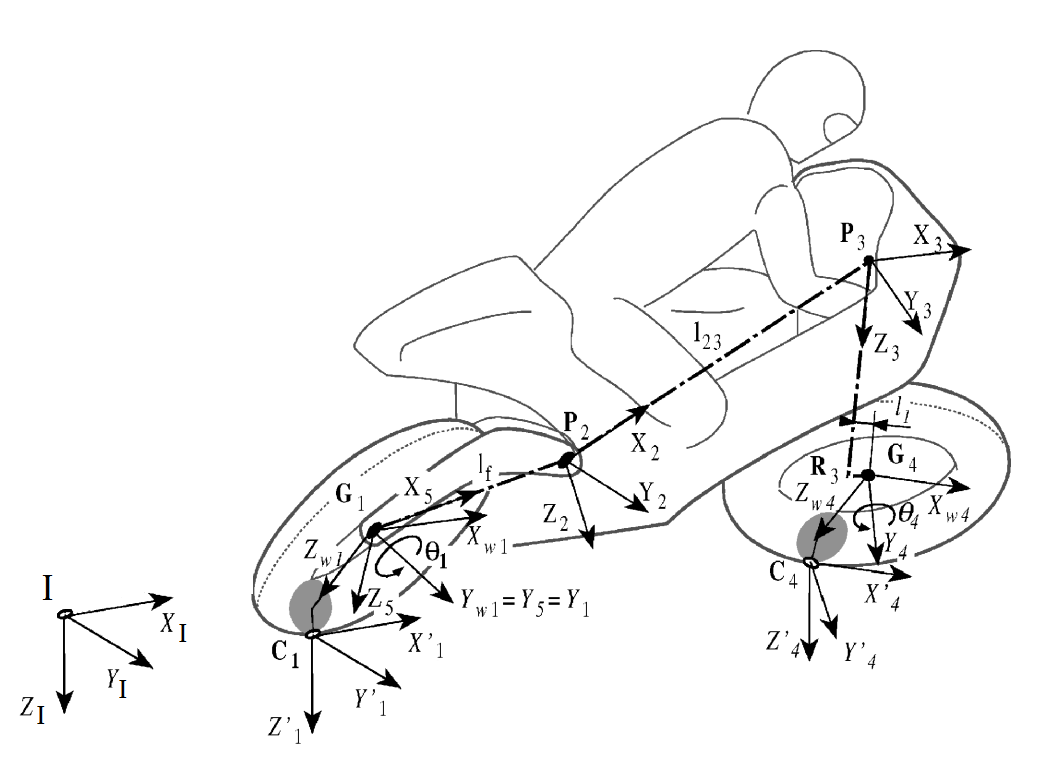
\includegraphics[width=0.85\textwidth]{abbildungen/05_Motorrad.png}
\caption{Motorrad als Mehrk\"orpersystem mit nat\"urlichen Koordinaten \cite[S. 10]{Cossalter2002}}
\label{fig:modell_motorrad}
\end{center}
\end{figure}
Das System wird mit Hilfe von zehn Koordinatensystemen beschrieben. Die Koordinatensysteme werden im Folgenden mit Hilfe ihrer zugeh\"origen homogenen Transformationsmatrizen identifiziert. Die Transformationsmatrizen $\matr{T}_{i}, i=1,\dots,10$ beinhalten jeweils eine Rotationsmatrix $\matr{R}_{i}$ und einen Ortsvektor $\vect{q}_{i}$ entsprechend \eqnref{gl:kos_transfHomog_homKoord_transfoKompl}, mit Hilfe derer ein \"Ubergang zum Inertialsystem $\KOS{I}$ m\"oglich ist. Die Komponenten von $\matr{R}_{i}$ und $\vect{q}_{i}$ sind die generalisierten Koordinaten des Systems. F\"ur zehn Koordinatensysteme werden daher, wie in Abschnitt \ref{sec:kos_natKoord} dargelegt wurde, \begin{align*}
12\cdot 10 &= 120
\end{align*} generalisierte Koordinaten eingef\"uhrt. Durch geeignete Festlegung der Einheitsvektoren der einzelnen Koordinatensysteme kann diese Zahl jedoch wesentlich reduziert werden. Auf einige dieser \"Uberlegungen wird im Folgenden Eingegangen. Die Bezeichnung einzelner Elemente weicht dabei von der Darstellung in \cite{Cossalter2002} ab, weil diese so einfacherer der Darstellung in \figureref{fig:modell_motorrad} zuzuordnen sind.  \hfill \newline
Das Inertialsystem wird durch die Einheitsvektoren ${\vect{c}_{x,I}=\transp{\left(1,0,0 \right)}}$ , ${\vect{c}_{y,I}=\transp{\left(0,1,0 \right)}}$ und ${\vect{c}_{z,I}=\transp{\left(0,0,1 \right)}}$ aufgespannt und durch den Ortsvektor ${\vect{O}=\transp{\left(0,0,0 \right)}}$ im Raum fixiert. Die Vektoren $\vect{c}_{x,I}$ und $\vect{c}_{y,I}$ bilden die Ebene, auf welcher sich das Motorrad bewegen kann. Die Einheitsvektoren der Koordinatensysteme werden so festgelegt, dass $\vect{u}_{i}$ in x-Richtung, $\vect{w}_{i}$ in y-Richtung und $\vect{v}_{i}$ in z-Richtung bez\"uglich $\KOS{I}$ positive Werte annehmen. \hfill \newline
Das Hinterrad wird durch drei Koordinatensysteme beschrieben. Zwei der Koordinatensysteme haben ihren Ursprung im Radmittelpunkt, das Dritte bewegt sich mit dem Kontaktpunkt zwischen Hinterreifen und Stra\ss{}e mit und wird durch $\matr{T}'_{1}$ identifiziert. Da dieser Kontaktpunkt in der Ebene, welche von $\vect{c}_{x,I}$ und $\vect{c}_{y,I}$ aufgespannt wird, liegen muss, ist die z-Komponente von $\vect{w}'_{1}$ konstant null. Der Vektor $\vect{v}'_{1}$ liegt des weiteren parallel zu $\vect{c}_{z,I}$ und ben\"otigt daher gar keine generalisierten Koordinaten.  Das Koordinatensystem $\matr{T}_{w1}$ ist so ausgerichtet, dass es in Fahrtrichtung zeigt. Der Einheitsvektor $\vect{u}_{w1}$ liegt parallel zur Fahrbahn und ben\"otigt daher keine variable z-Komponente. Die x-Achsen von $\matr{T}'_{1}$ und $\matr{T}_{w1}$ werden au\ss{}erdem als parallel definiert, wodurch drei weitere generalisierte Koordinaten obsolet werden. Da alle Koordinatensysteme normierte Rechtssysteme sein sollen stehen die Vektoren $\vect{u}'_{1}, \vect{w}'_{1}$ senkrecht aufeinander. Das System $\matr{T}'_{1}$ liegt weiterhin in einer konstanten Ebene, wodurch f\"ur die Definition von $\vect{u}'_{1}, \vect{w}'_{1}$ bereits zwei generalisierte Koordinaten ausreichen. $\matr{T}_{1}$ ist fest mit dem Hinterrad verankert und geht aus $\matr{T}_{w1}$ direkt durch Drehung um die $Y_{w1}$ Achse hervor. Diese Drehung ben\"otigt nur eine generalisierte Koordinate. Da beide Systeme den gleichen Ursprung haben, entfallen weitere drei generalisierte Koordinaten. Insgesamt stellt man fest, dass sich diese drei Koordinatensysteme durch deren geschickte Definition mit Hilfe von 15 anstelle von $12\cdot 3 = 36$ generalisierten Koordinaten $\vect{q}$ beschreiben lassen. \begin{align*}
\intertext{F\"ur $\matr{T}_{w1}$ gilt}
\vect{u}_{w1}&=\transp{\left(u_{w1,x}, u_{w1,y},0,0 \right)} 
\\
\vect{w}_{w1}&=\transp{\left(w_{w1,x}, w_{w1,y}, w_{w1,z}, 0\right)}
\\
\vect{v}_{w1}&=\transp{\left(v_{w1,x}, v_{w1,y}, v_{w1,z}, 0\right)}
\\
\vect{q}_{w1}&=\transp{\left(q_{w1,x}, q_{w1,y}, q_{w1,z}, 1\right)}.
\intertext{F\"ur $\matr{T}'_{1}$ gilt}
\vect{u}'_{1}&=\vect{u}_{w1}
\\
\vect{w}'_{1}&=\transp{\left(-u_{w1,y}, u_{w1,x}, 0, 0\right)}
\\
\vect{v}'_{1}&=\transp{\left(0, 0, 1, 0\right)}
\\
\vect{q}'_{1}&=\transp{\left(q'_{1,x}, q'_{1,y}, q'_{1,z}, 1\right)}.
\intertext{F\"ur $\matr{T}_{1}$ gilt}
\matr{T}_{1}&= \inv{\matr{T}_{rot,w1}}\matr{T}_{w1} ,
\intertext{wobei die Rotation um die Achse $Y_{w1}$ mit}
\matr{T}_{rot,w1}&=\begin{pmatrix}
\cos \left( \theta_{1}
 \right) &0&\sin \left( \theta_{1}  \right) &0\\
0&1&0&0\\ -\sin \left( \theta_{
1}   \right) &0&\cos \left( \theta_{1}  \right) &0\\ 
 0&0&0&1\end{pmatrix} 
\intertext{erfolgt.}
\intertext{F\"ur den Vektor der generalisierten Koordinaten ergibt sich damit}
\vect{q}= &\left(u_{w1,x}, u_{w1,y},w_{w1,x}, w_{w1,y}, w_{w1,z}, v_{w1,x}, v_{w1,y}, v_{w1,z},\right. \\
 & \left. q_{w1,x}, q_{w1,y}, q_{w1,z}, q'_{1,x}, q'_{1,y}, q'_{1,z}, \theta_{1}  \right)^{T}
\end{align*}
Diese \"Uberlegungen gelten f\"ur das Vorderrad analog, wobei sich das Rad nat\"urlich mit der Lenkachse mit dreht. Die Richtungsvektoren $\vect{w}_{3}$ und $\vect{w}_{w4}$ sind daher gleich.\hfill \newline
Die \"ubrigen vier Koordinatensysteme beschreiben die Lage der Hinterradschwinge, die Lenkerposition und die Lage der unged\"ampften Vorderradmassen. Die Hinterradschwinge wird mit Hilfe von $\matr{T}_{5}$ und $\matr{T}_{2}$ beschrieben. $\matr{T}_{5}$ hat seinen Ursprung an der gleichen Stelle wie $\matr{T}_{w1}$. Die x-Achse zeigt jedoch nicht gerade nach vorn, sondern auf das Gelenk, in welchem die Hinterradschwinge mit dem Motorradrahmen verbunden ist. Die Y-Achse von $\matr{T}_{5}$ ist identisch mit der von $\matr{T}_{w1}$. F\"ur die Beschreibung von $\matr{T}_{5}$ werden daher sechs neue generalisierte notwendig. $\matr{T}_{2}$ hat den Ursprung in der Rahmenaufh\"angung der Hinterradschwinge und eine y-Achse, welche zu der von $\matr{T}_{w1}$ parallel ist. Die Richtungsvektoren dieser Achse sind daher identisch. Die x-Achse von $\matr{T}_{2}$ ist so ausgerichtet, dass sie senkrecht auf der Lenkachse steht. Die zur Beschreibung dieser zwei Systeme notwendigen Vektoren lauten daher \begin{align*}
\vect{u}_{2}&=\transp{\left(u_{2,x}, u_{2,y},u_{2,z},0 \right)} 
\\
\vect{w}_{2}&=\vect{w}_{w1}
\\
\vect{v}_{2}&=\transp{\left(v_{2,x}, v_{2,y}, v_{2,z}, 0\right)}
\\
\vect{q}_{2}&=\transp{\left(q_{2,x}, q_{2,y}, q_{2,z}, 1\right)}
\intertext{f\"ur $\matr{T}_{2}$ und}
\vect{u}_{5}&=\transp{\left(u_{5,x}, u_{5,y}, u_{5,z}, 0\right)}
\\
\vect{w}_{5}&=\vect{w}_{w1}
\\
\vect{v}_{5}&=\transp{\left(v_{5,x}, v_{5,y}, v_{5,z}, 0\right)}
\\
\vect{q}_{5}&=\vect{q}_{w1}
\intertext{f\"ur $\matr{T}_{5}$.}
\end{align*} Das System $\matr{T}_{3}$ wird so ausgerichtet, dass die z-Achse entlang der Lenkachse verl\"auft. Der Ursprung liegt im Schnittpunkt der Lenkachse mit der auf der Lenkachse senkrecht stehenden Ebene, welche den Ursprung von $\matr{T}_{2}$ als Element hat. Die Elemente von $\matr{T}_{3}$ lauten damit \begin{align*}
\vect{u}_{3}&=\transp{\left(u_{3,x}, u_{3,y}, u_{3,z}, 0\right)}
\\
\vect{w}_{3}&=\transp{\left(w_{3,x}, w_{3,y}, w_{3,z}, 0\right)}
\\
\vect{v}_{3}&=\vect{v}_{2}
\\
\vect{q}_{3}&=\transp{\left(q_{3,x}, q_{3,y}, q_{3,z}, 1\right)}.
\end{align*} 
Das letzte Koordinatensystem umfasst die unged\"ampften Massen am Vorderrad. Es ben\"otigt keine neuen generalisierten Koordinaten, da es sich mit Ausnahme der Rotation mit dem Vorderrad mitbewegt. \hfill \newline
Insgesamt ergeben sich durch die so definierten Koordinatensysteme also $51$ generalisierte Koordinaten welche sich aus $15$ generalisierten Koordinaten f\"ur das Hinterrad, $15$ f\"ur die Schwinge, $9$ f\"ur den Lenker und $12$ f\"ur das Vorderrad zusammen setzen. Die vorl\"aufig berechnete Anzahl von 120 Koordinaten konnte also durch geeignete Festlegung der Koordinatensysteme zueinander um mehr als die h\"alfte reduziert werden. \hfill \newline

Die Anzahl generalisierter Koordinaten ist immer noch ziemlich hoch. In Folge der Modellierung mit nat\"urlichen Koordinaten lassen sich aber im n\"achsten Schritt die Zwangsbedingungen auf sehr einfache Art formulieren. Wie im Abschnitt \ref{sec:kos_natKoord} dargelegt wurde, m\"ussen alle Vektoren $\vect{u}_{i}, \vect{w}_{i}, \vect{v}_{i}$ Einheitsl\"ange haben und senkrecht aufeinander stehen. Diese Bedingungen lassen sich auf triviale Weise mit dem Skalarprodukt formulieren. Stellt man diese Bedingungen f\"ur alle eingef\"uhrten Richtungsvektoren auf, so ergeben sich 26 Zwangsbedingungen. Mit Hilfe weiterer Gleichungen kann die Geometrie des Motorrads beschrieben werden.\hfill \newline
Beispielhaft sei die konstante L\"ange der Hinterradschwinge betrachtet. Durch die geschickte Wahl der Koordinatenurspr\"unge von $\matr{T}_{w1}$ und $\matr{T}_{2}$ ist die Gleichung sehr einfach aufzustellen. Sei die Schwingenl\"ange durch den Parameter $l_{schw}$ gegeben. Die geforderte konstante L\"ange l\"asst sich dann mit dem Skalarprodukt als \begin{align*}
\skalar{\vect{q}_{2}-\vect{q}_{w1}}{\vect{q}_{2}-\vect{q}_{w1}} - l_{schw}^{2}&=0
\end{align*} formulieren. Dabei ist darauf zu achten, dass die Zwangsbedingung der Form $\phi\of{\vect{q}}=0$ entspricht. Auf \"ahnliche Weise lassen sich sieben weitere geometrische Beziehungen als Zwangsbedingungen formulieren. Dabei sind alle Gleichungen frei von trigonometrischen Funktionen. In Folge dessen l\"asst sich die Jacobimatrix der Zwangsbedingungen $\Phi_{\vect{q}}\of{\vect{q}}$ einfach berechnen. \hfill \newline
Die generalisierten Koordinaten k\"onnten mit Hilfe der Zwangsbedingungen auf einen Satz Minimalkoordinaten reduziert werden. Dieser Ansatz ist aber nicht zweckm\"a\ss{}ig, da der Rechenaufwand f\"ur die algebraische Umformung sehr hoch ist und die erhaltenen Ausdr\"ucke f\"ur die Minimalkoordinaten sehr komplex w\"aren. Daher verwendet man zur L\"osung des Systems den Ansatz von Langrange \mbox{2. Art}, wie er in \eqnref{gl:mech_lagrange2ArtDefCossalter} angegeben ist. \hfill \newline

Der zur L\"osung von \eqnref{gl:mech_lagrange2ArtDefCossalter} ben\"otigte Ausdruck f\"ur die kinetische Energie wurde bereits in Abschnitt \ref{ssec:mech_lag2_kinEn} ausf\"uhrlich hergeleitet. Mit Hilfe der generalisierten Koordinaten, den Schwerpunktkoordinaten und den Elementen des Tr\"agheitstensors kann die Gleichung f\"ur die kinetische Energie nach \eqnref{gl:mech_lag2_kinEn_kinEnHomogAllg} direkt aufgestellt werden. Dabei ist lediglich darauf zu achten, dass nur die Systeme $\matr{T}_{w1}, \matr{T}_{2}, \matr{T}_{3}, \matr{T}_{w4}, \matr{T}_{5}$ und $\matr{T}_{6}$ in diese Gleichung eingehen. Die \"ubrigen vier Koordinatensysteme werden ausschlie\ss{}lich zur Beschreibung der Reifenbewegung und der Reifenkr\"afte ben\"otigt. \hfill \newline

Die Formulieren der virtuellen Arbeit und die Umformung zu generalisierten Kr\"aften ist keine triviale Aufgabe. Als Beispiel sollen die virtuelle Arbeit der Gravitation, der Reifenkr\"afte und Reifenmomente erl\"autert werden.  \cite[S.14 f.]{Cossalter2002}

\begin{itemize}
\item Gravitation
\item Reifenkr\"afte
\item Reifenmomente
\end{itemize}

Umformung und L\"osung der Gesamtgleichung entsprechend Abschnitt \ref{sec:mech_dae}.